\chapter{Gegevensstructuren voor strings}
\section{Inleiding}
\begin{itemize}
    \item Efficiënte gegevensstructuren kunnen een zoeksleutel lokaliseren door elementen één voor één te testen.
    \item Dit heet \textbf{radix search}.
    \item Meerdere soorten boomstructuren die radix search toepassen.
    \begin{itemize}
        \item \textbf{Digitale zoekbomen}: deze bomen hebben als nadeel dat de zoeksleutels nie noodzakelijk in de volgorde voorkomen dat ze toegevoegd zijn.
        \item \textbf{Tries}: tries houden wel rekening met de toevoegvolgorde.
        \item \textbf{Ternaire zoekbomen}: een alternatieve voorstelling van een meerwegstrie, die minder geheugen gebruikt en toch efficiënt blijft.
    \end{itemize}
    \alert Veronderstel dat geen enkele sleutel een prefix is van een ander.

    De sleutels \texttt{test} en \texttt{testen} zullen dus nooit samen voorkomen in de boom aangezien \texttt{test} een prefix is van \texttt{testen}. Dit is noodzakelijk: stel dat een langere sleutel reeds in de boom zit. Als de kortere sleutel gezocht wordt, of willen toevoegen, zullen er uiteindelijk geen sleutelelementen overblijven om ze te onderscheiden.
\end{itemize}

\section{Digitale zoekbomen}
\begin{itemize}
    \item Sleutels worden opgeslagen in de knopen.
    \item Zoeken en toevoegen verloopt analoog als een normale binaire zoekboom.
    \item Slechts één verschil: 
    \begin{itemize}
        \item De juiste deelboom wordt niet bepaald door de zoeksleutel te vergelijken met de sleutel in de knoop.
        \item Wel door enkel het volgende element (van links naar rechts) te vergelijken.
        \item Bij de wortel wordt het eerste sleutelelement gebruikt, een niveau dieper het tweede sleutelelement, enz.
    \end{itemize}
    \item In de cursus zijn de sleutelelementen beperkt tot bits $\rightarrow$ \textbf{binaire digitale zoekbomen}.
    \item Bij een knoop op diepte $i$ wordt bit $(i + 1)$ van de zoeksleutel gebruikt om af te dalen in de juiste deelboom.
    \alert De zoekboom overlopen in inorder levert de zoeksleutels niet noodzakelijk in volgorde op.
    \begin{itemize}
        \item Sleutels in de linkerdeelboom van een knoop op diepte $i$ zijn zeker kleiner dan deze in de rechterdeelboom.
        \item Maar, de sleutel van de knoop kan toch in beide deelbomen terechtkomen.
    \end{itemize}
    \item De hoogte van een digitale zoekboom wordt bepaald door het aantal bits van de langste sleutel.
    \item Performantie is vergelijkbaar met rood-zwarte bomen:
    \begin{itemize}
        \item Voor een groot aantal sleutels met relatief kleine bitlengte is het zeker beter dan een binaire zoekboom en vergelijkbaar met die van een rood-zwarte boom.
        \item Het aantal vergelijkingen is nooit meer dan het aantal bits van de zoeksleutel.
        \good Implementatie van een digitale zoekboom is eenvoudiger dan die van een rood-zwarte boom.
        \alert De beperkende voorwaarde is echter dat er efficiënte toegang nodig is tot de bits van de sleutels.
    \end{itemize}
\end{itemize}

\section{Tries}
\begin{itemize}
    \item Een digitale zoekstructuur die wel de volgorde van de opgeslagen sleutels behoudt.
\end{itemize}

\subsection{Binaire tries}

\begin{figure}[ht]
    \centering
    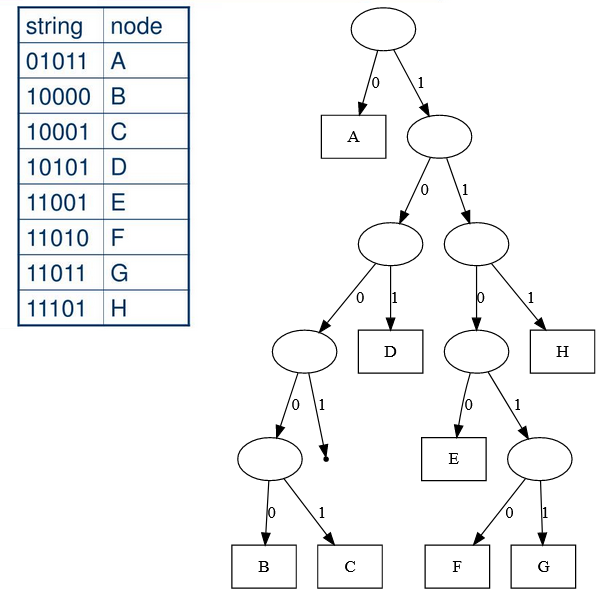
\includegraphics[width=\textwidth]{binary_trie}
    \caption{Een voorbeeld van een binaire trie met opgeslagen sleutels $A$, $B$, $C$, $D$, $E$, $F$, $G$ en $H$. Elk van deze sleutels heeft een (willekeurige) bitrepresentatie die de individuele elementen van de sleutels voorstelt. De zoekweg van de sleutel $E$ wordt aangegeven door rode verbindingen.}
    \label{fig:binary_trie}
\end{figure}

\begin{itemize}
    \item Zoekweg wordt bepaald door de opeenvolgende bits van de zoeksleutel.
    \item Sleutels worden enkel opgeslaan in de bladeren.
    \begin{itemize}
        \item  De boom \textit{inorder} overlopen geeft de sleutels gerangschikt terug.
        \item  De zoeksleutel moet niet meer vergeleken worden met elke knoop op de zoekweg. 
    \end{itemize}
    \item Twee mogelijkheden bij \textbf{zoeken} en \textbf{toevoegen}:
    \begin{enumerate}
        \item Indien een lege deelboom bereikt wordt, bevat de boom de zoeksleutel niet. De zoeksleutel kan dan in een nieuw blad op die plaats toegevoegd worden.
        \item Anders komen we in een blad. De sleutel in dit blad \textbf{kan} eventueel gelijk zijn aangezien ze zeker dezelfde beginbits hebben.  

        \begin{itemize}
            \item Als we bijvoorbeeld \texttt{10011} zoeken maar de boom bevat enkel de sleutel \texttt{10010}, zullen we in het blad met de sleutel \texttt{10010} uitkomen aangezien de eerste 4 elementen hetzelfde zijn. De sleutels zijn echter niet gelijk.
            \item Indien de sleutels niet hetzelfde zijn, kunnen twee mogelijkheden voorkomen:
            \begin{enumerate}
                \item \textbf{Het volgende bit verschilt.} Het blad wordt vervangen door een knoop met twee kinderen die de twee sleutels bevat.
                \item \textbf{Een reeks van opeenvolgende bits is gelijk.} Het blad wordt vervangen door een reeks van inwendige knopen, zoveel als er gemeenschappelijke bits zijn. Bij het eerste verschillende krijgen we terug het eerste geval.
            \end{enumerate}
        \end{itemize}
    \end{enumerate}
    \alert Wanneer opgeslagen sleutels veel gelijke bits hebben, zijn er veel knopen met één kind.
    \begin{itemize}
        \item Het aantal knopen is dan ook hoger dan het aantal sleutels.
        \item Een trie met $n$ gelijkmatige verdeelde sleutels heeft gemiddeld $n/\ln 2 \approx 1.44n$ inwendige knopen.
    \end{itemize}
    \item De structuur is onafhankelijk van de toevoegvolgorde van de sleutels.
    \item De sleutels in de zoekweg worden enkel getest op de bit die op dat niveau van toepassing is.
\end{itemize}


\subsection{Meerwegstries}
\begin{itemize}
    \item Heeft als doel de hoogte van een trie met lange sleutels te beperken.
    \item Meerdere sleutelbits in één enkele knoop vergelijken.
    \item Een sleutelelement kan $m$ verschillende waarden aannemen, zodat elke knoop (potentiaal) $m$ kinderen heeft $\rightarrow$ $m$-wegsboom.
    \item \textbf{Zoeken} en \textbf{toevoegen} verloopt analoog als bij een binaire trie:
    \begin{itemize}
        \item In elke knoop moet nu enkel een $m-$wegsbeslissing genomen worden, op basis van het volgende sleutelelement.
        \item Dit kan in $O(1)$ door per knoop een tabel naar wijzers van de kinderen bij te houden, geïndexeerd door het sleutelelement.
    \end{itemize}
    \item Ook hier is de structuur onafhankelijk van de toevoegvolgorde van de sleutels, en de boom in inorder overlopen zorgt ook voor een gerangschikte lijst.
    \item De performantie is ook analoog met die van binaire tries.
    \begin{itemize}
        \item Zoeken of toevoegen van een willekeurige sleutel vereist gemiddeld $O(\log_m n)$ testen op het aantal sleutelelementen.
        \item De boomhoogte wordt ook beperkt door de lengte van de langste opgeslagen sleutel.
        \item Er zijn gemiddeld $n/\ln m$ inwendige knopen.
        \item Het aantal wijzers per knoop is wel $mn \ln m$.
    \end{itemize}
    \item Wat als we toch willen toelaten dat een sleutel een prefix van een andere sleutel mag zijn?
    \begin{itemize}
        \item In een meerwegstrie kan dit opgelost worden door elke sleutel af te sluiten met een speciaal sleutelelement, dat in geen enkele andere sleutel voorkomt.
    \end{itemize}
    \alert Het grootste nadeel is dat meerwegstries veel geheugen gebruiken. Mogelijke verbeteringen zijn:
    \begin{itemize}
        \item In plaats van een tabel met $m$ wijzers te voorzien, waarvan de meeste toch nullwijzers zijn, kan een gelinkte lijst bijgehouden worden. Elk element van de gelinkte lijst bevat een sleutelelement en een wijzer naar een kind. De lijst is ook gerangschikt volgens de sleutelelementen, zodat niet altijd de hele lijst moet onderzocht worden om het juiste element te vinden.
        
        Op  de hogere niveaus is een tabel met $m$ wijzers toch beter, omdat daar meer kinderen kunnen zijn.
        \item Een trie kan ook enkel voor de eerste niveaus gebruikt worden, en daarna een andere gegevensstructuur gebruiken. Vaak stopt men als een deelboom niet meer dan $s$ sleutels bevat. Deze sleutels worden dan opgeslaan in een korte lijst, die dan sequentieel doorzocht kan worden. Het aantal inwendige knopen daalt met een factor $s$, tot ongeveer $n/(s \ln m)$.
    \end{itemize}
\end {itemize}

\section{Variabelelengtecodering}
\begin{itemize}
    \item Normaal worden gegevens opgeslaan  in gegevensvelden met een vaste grootte.
    \begin{itemize}
        \item Een karakter in ASCII-codering wordt bevat altijd 7 bits.
        \item Een integer datastructuur voorziet altijd 32 bits.
    \end{itemize}
    \item Soms is het nuttig om variabele lengte te voorzien:
    \begin{enumerate}
        \item \textbf{Verhoogde flexibiliteit}: Wanneer blijkt dat er meer bits nodig zijn, is het eenvoudig om meer bits te voorzien. 
        \item \textbf{Compressie}: Veelgebruikte letters kunnen een kortere bitlengte krijgen om de grootte van de totale gegevens te reduceren.
    \end{enumerate}
    \item In beide gevallen hebben we een \textbf{alfabet}, waarbij we niet elke letter door evenveel bits laten voorstellen.
    \alert Een belangrijk nadeel is dat eerst de hele codering ongedaan moet gemaakt worden vooraleer er in gezocht kan worden. Variabelelengtecodering is dan ook enkel nuttig als dit niet uitmaakt.
    \item Bij het \textbf{decoderen} is er een \textbf{prefixcode}. 
    \begin{itemize}
        \item Dit is een codering waarbij een \textbf{codewoord}, nooit het prefix van een ander codewoord kan zijn.
        \item Een code is een mapping die elke letter van het alfabet afbeeldt op een codewoord. Bijvoorbeeld, de letters $A$, $B$, $C$ en $D$ kunnen volgende codewoorden krijgen:
        \begin{align*}
            A &\rightarrow 0 \\
            B &\rightarrow 1 \\
            C &\rightarrow 01 \\
            D &\rightarrow 11 \\
        \end{align*}
        \item Op die manier weten we dat het einde van een codewoord is bereikt zonder het begin van het volgende codewoord te moeten analyseren.
        \item Een typische prefixcode voor natuurlijke getallen schrijft het getal op in een 128-delig stelsel en elk cijfer wordt apart opgeslaan in een aparte byte. Bij het laatste cijfer wordt er 128 opgeteld, zodat de laatste byte een 1-bit heeft op de meest significante plaats.
        \item In geschreven taal wordt er gewacht tot een spatie of leesteken tegengekomen wordt om het onderscheidt tussen verschillende woorden te maken.
    \end{itemize}
    \item Een trie is geschikt om een invoerstroom te decoderen die gecodeerd is met een prefixcode.
    \begin{itemize}
        \item Alle codewoorden worden eerst opgeslaan in de trie.
        \item Aan het begin van een codewoord starten we bij de wortel.
        \item Per ingelezen bit of byte (afhankelijk van het probleem, bij strings zeker een byte) gaan we een niveau omlaag in de trie.
        \item Bij een blad is het codewoord compleet.
    \end{itemize}
\end{itemize}

\subsection{Universele codes}
\begin{itemize}
    \item Deze codes zijn onafhankelijk van de gekozen brontekst.
    \item De codes worden hier geïllustreerd als de codering voor de verschillende positieve gehele getallen.
\end{itemize}

\begin{table}[ht]
    \centering
    \begin{tabular}{|r | l | l | l |}
        \hline
        & Elias' gammacode & Elias' deltacode & Fibonaccicode \\
        \hline
        1 & 1 & 1 & 11  \\
        2 & 010 & 0100 & 011 \\
        3 & 011 & 0101 & 0011  \\
        4 & 00100 & 01100 & 1011  \\
        5 & 00101 & 01101 & 00011  \\
        6 & 00110 & 01110 & 10011  \\
        7 & 00111 & 01111 & 01011  \\
        8 & 0001000 & 00100000 & 000011  \\
        9 & 0001001 & 00100001 & 100011  \\
        ... &  &  &   \\
        23 & 000010111 & 001010111 & 01000011  \\
        ... &  &  &   \\
        45 & 00000101101 & 0011001101 & 001010011  \\
        ... &  &  &   \\

        \hline
    \end{tabular}
\end{table}

\subsubsection{De Elias' gammacode}
\begin{itemize}
    \item Gegeven een getal $n$:
    \begin{itemize}
        \item Stel het getal voor met zo weinig mogelijk bittekens ($k$) en laat dit voorafgaan door $k - 1$ nulbits.
        \item Een getal $n$ wordt voorgesteld door $2\lfloor \log_2 n\rfloor + 1$ bittekens.
        \item Anders gezegd: zet $n$ om in zijn binaire representatie. Deze representatie heeft $k$ bits. Laat deze representatie voorafgaan door $k - 1$ nulbits.
    \end{itemize}
\end{itemize}

\subsubsection{De Elias' deltacode}
\begin{itemize}
    \item Gegeven een getal $n$:
    \begin{itemize}
        \item Gebruik de laatste $k-1$ bittekens van het getal en laat dit voorafgaan door de Elias' gammacode voor $k$.
        \item Een getal $n$ wordt voorgesteld door $\lfloor \log_2 n\rfloor  + 2\lfloor \log_2(\log_2 n + 1)\rfloor + 1$ bittekens.
    \end{itemize}
\end{itemize}

\subsubsection{De Fibonaccicode}
\begin{itemize}
    \item De Fibonaccireeks
    $$1, 2, 3, 5, 8, 13, 21, 34, 55, 89, 144, 233, 377, 610, ...$$
    \item Dit heeft als eigenschap dat een getal $i$ geschreven kan worden als de som van verschillende Fibonaccigetallen zodanig dat er nooit twee getallen in de reeks worden gebruikt die onmiddellijke buren zijn van elkaar.
    \item Gegeven een getal $n$:
    \begin{itemize}
        \item Overloop de Fibonaccireeks van klein naar groot en gebruik een éénbit voor elk getal dat in de berekende som voorkomt, en een nulbit voor alle andere getallen. Op het einde komt er altijd een éénbit. 
        \item Een getal $n$ wordt voorgesteld door $k + 1$ bittekens.
    \end{itemize}
\end{itemize}

\section{Huffmancodering}
\begin{itemize}
    \item Sommige letters in een tekst kunnen meer voorkomen dan een andere.
    \item Minder bittekens gebruiken voor die letters speelt ten voordele van de grootte van de hele tekst.
\end{itemize}

\subsection{Opstellen van de decoderingsboom}
\begin{figure}[ht]
    \centering
    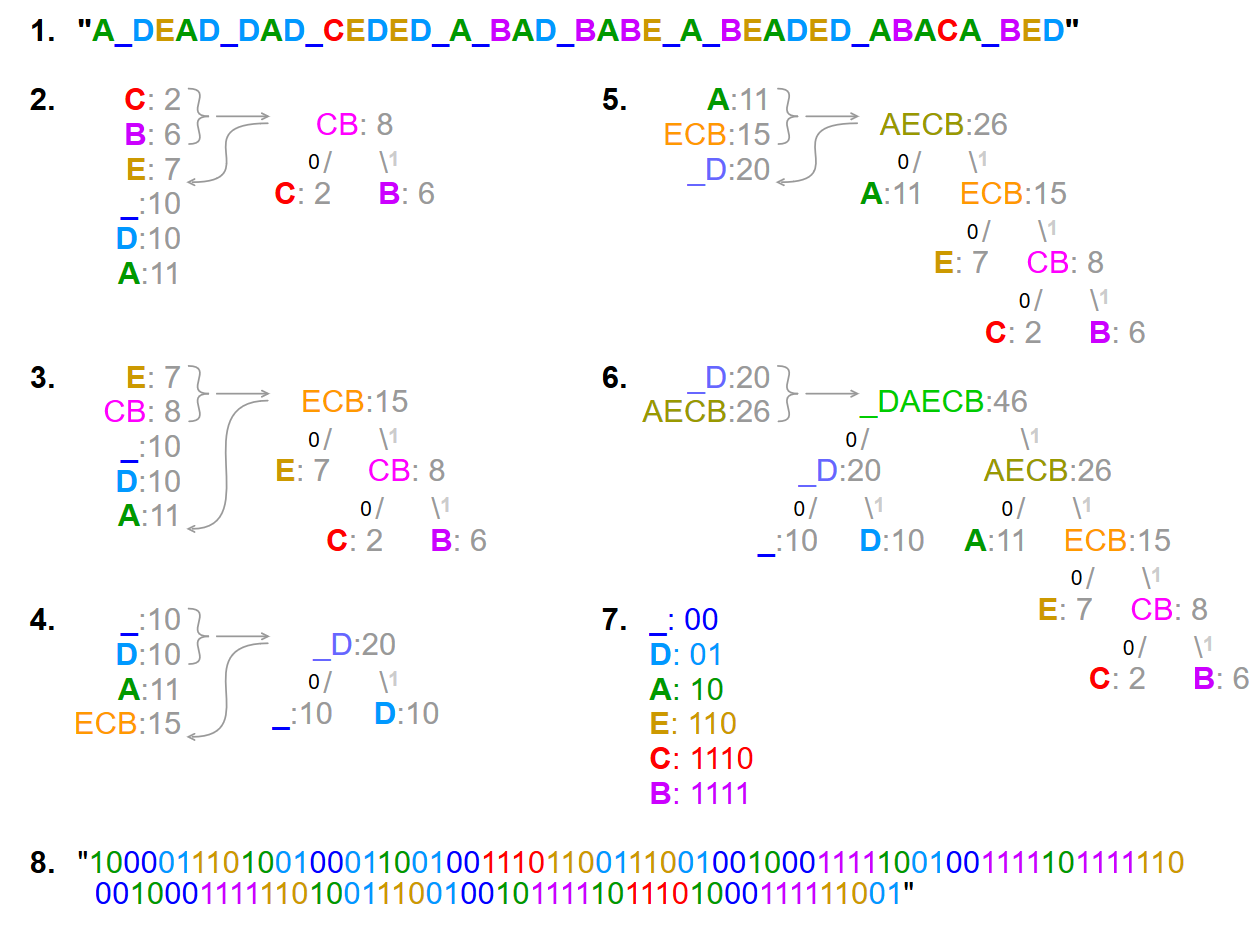
\includegraphics[width=\textwidth]{huffman_coding}
    \caption{Een visualisatie van huffmancodering, maar met een gewone binaire boom en \textbf{niet met een trie}. De te coderen tekst wordt weergegeven bij stap 1. 
    In stap 2 wordt eerst elke letter wordt gesorteerd in een lijst bijgehouden (eigenlijk een bos van bomen) volgens zijn niet-stijgende frequenties $f_i$. Stap 2 tot 6 neemt dan altijd de twee minst frequente bomen en combineert ze om een nieuwe boom te bekomen. Die boom wordt terug in het bos gestoken. Stap 7 toont de werkelijke codering. Stap 8 toont de gecodeerde versie van de tekst in stap 1.}
    \label{fig:huffman_coding}
\end{figure}
\begin{itemize}
    \item Er wordt een prefixcode toegepast waarbij elke letter een apart codewoord krijgt die voor de hele tekst geldt.
    \item We zullen bitcodes gebruiken, en dan ook een binaire trie.
    \item Om de optimale code op te stellen moet nagegaan worden hoe vaak elk codewoord gebruikt zal worden.
    \item Er is een alfabet $\Sigma = \{s_i | i = 0, ..., d - 1\}$
    \item We bekomen de frequenties $f_i$ door elke letter $s_i$ te tellen in de tekst.
    \item We zoeken een trie met $n$ bladeren die de optimale code oplevert.
    \begin{itemize}
        \item Neem een willekeurige binaire trie met $d$ bladeren, elk met een letter uit $\Sigma$.
        \item Ken aan elke knoop een gewicht toe:
        \begin{itemize}
            \item Een blad krijgt als gewicht de frequentie $f_i$ van de overeenkomstige letter.
            \item Een inwendige knoop krijgt als gewicht de som van de gewichten van zijn kinderen.
        \end{itemize}
        \item Stel dat het bestand gecodeerd wordt met de bijhorende code en dat deze trie gebruikt wordt om te decoderen.
        \item Het totaal aantal bits in het gecodeerde bestand is de som van de gewichten van alle knopen samen, met uitzondering van de wortel.
        \item De wortel heeft gewicht $n$ (de som van alle frequenties), dus we zoeken een trie waarvoor $n$ minimaal wordt.
    \end{itemize}
    \item Stel een knoop $k$ met gewicht $w_k$ op diepte $d_k$. en een knoop $l$ met gewicht $w_l$ op diepte $w_l$, zodanig dat $k$ niet onder $l$ hangt en $l$ niet onder $k$.
    \item Er kan een nieuwe trie gemaakt worden $k$, inclusief de bijbehorende deelboom, van plaats te verwisselen met $l$.
    \begin{itemize}
        \item Er waren $d_k$ knopen boven $k$ in de trie, die verliezen gewicht $w_k$ maar krijgen gewicht $w_l$.
        \item Er waren $d_l$ knopen boven $l$ in de trie, die verliezen gewicht $w_l$ maar krijgen gewicht $w_k$.
    \end{itemize}
    \item De totale gewichtsverandering van de totale trie is 
    $$(d_k - d_l)(w_l - w_k)$$
    \item Als $l$ een groter gewicht en kleinere diepte dan $k$ heeft, is er een betere trie bekomen.
    \item De optimale trie heeft volgende eigenschappen:
    \begin{itemize}
        \item Geen enkele knoop heeft een groter gewicht dan een knoop op een kleinere diepte.
        \item Geen enkele knoop heeft een groter gewicht dan een knoop links (of rechts) van hem op dezelfde diepte, want dan kunnen de twee knopen omgewisseld worden.
    \end{itemize}
    \item Constructie van de coderingsboom: (dunno actaully)
    \begin{itemize}
        \item Op elk moment is er een bos van deelbomen die aan elkaar gehangen moeten worden.
        \item In het begin bestaat het bos uit enkel bladeren.
        \item Er worden twee bomen uit het bos gehaald en worden verenigd onder een nieuwe knoop en wordt terug in het bos gestoken.
        \item De diepte $h$ van de boom is onbekend, maar wel weten we dat:
        \begin{itemize}
            \item alle knopen op niveau $h$ zijn zeker bladeren,
            \item dat $h$ een even getal is.
        \end{itemize}
        \item We kunnen bladeren twee aan twee samen nemen, telkens de lichtste (kleinst gewicht)  die overblijven.
        \item De resulterende bomen hebben altijd een groter gewicht, dus komen later in het gerangschikte bos.
        \item Dit blijft herhaald worden tot dat er maar één boom overblijft (stap 2 tot 6 in figuur \ref{fig:huffman_coding}).
    \end{itemize}
\end{itemize}

\subsection{Patriciatries}
\begin{figure}[ht]
    \centering
    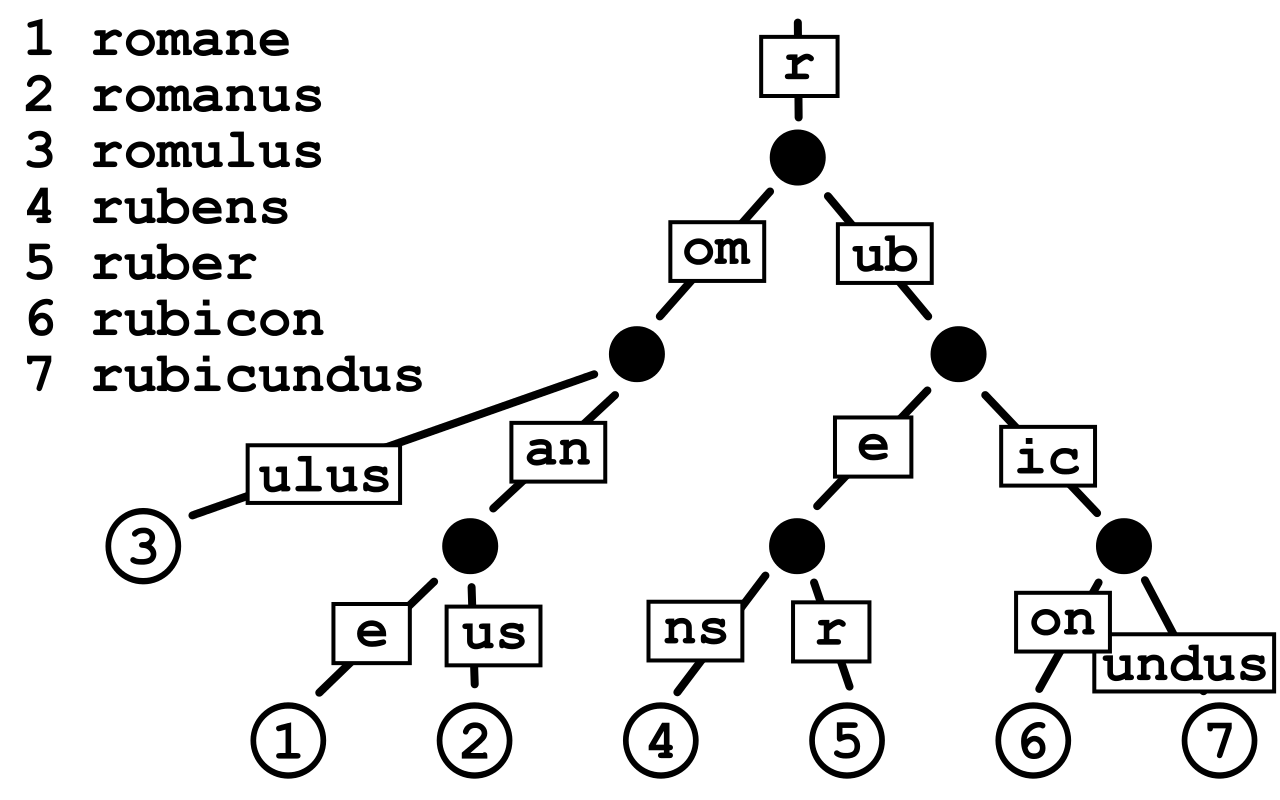
\includegraphics[width=0.5\textwidth]{patriciatrie}
    \caption{Een patriciatrie. Elk blad bevat een verwijzing naar een woord in een lijst en knopen met maar één kind worden samengevoegd.}
    \label{fig:patriciatrie}
\end{figure}
\begin{itemize}
    \alert Veel trieknopen hebben maar één kind zodat er veel ongebruikt geheugen is.
    \alert Er zijn ook twee soorten knoopen: inwendige knoop zonder sleutel maar met wijzers naar kinderen, en bladeren met sleutel maar zonder wijzers naar kinderen.
    \item Een \textbf{Patriciatrie} (Practical Algorithm to Retrive Information Coded In Alphanumeric) verwijdert deze problemen door enkel \textbf{knopen met meer dan één kind te behouden}.
    \item Bij een gewone meerwegstrie kunnen knopen voorkomen met maar één kind.
    \item Zo een knoop kan weggelaten worden en zijn kind kan in de plaats gezet worden.
    \item Twee gevolgende:
    \begin{enumerate}
        \item Als we in een kind komen, moeten we weten hoeveel voorouders er ontbreken. Dit lossen we op door een \textbf{testindex} in de knoop bijhouden, de index van het te testen karakter.
        \item De karakters die niet getest worden kunnen tot conflict leiden bij een zoekstring waarbij die karakters niet overeenkomen.
    \end{enumerate}
    \item Een knoop is \textbf{expliciet} als hij nog voorkomt in de boom.
    \item Een knoop is \textbf{impliciet} als hij enkel wordt aangeduid door een indexsprong aangegeven in de nakomeling.
    \item We gaan ervan uit dat de trie \textbf{niet ledig} is.
    \item \textbf{Zoeken.}
    \begin{itemize}
        \item Test altijd op het karakter aangegeven door de testindex.
        \item Als dit leidt naar een nulpointer zit de string niet in de boom.
        \item Als we in een blad komen, weten we niet zeker of dat dit de gezochte string is: karakters die niet getest zijn kunnen verschillen.
        \item Dus in een blad wordt de zoekstring compleet vergeleken met de string die in het blad zit.
    \end{itemize}
    \item \textbf{Toevoegen.}
    \begin{itemize}
        \item Het kan zijn dat we een blad moeten toevoegen aan een implicite knoop.
        \item We houden een \textbf{verschilindex} bij die de eerste plaats aanduidt waar de nieuwe string verschilt van de meest gelijkende string in de trie (deze met de langst gemeenschappelijke prefix).
        \item De zoekoperatie eindigt altijd in een explicite knoop. Er zijn dan drie mogelijkheden als de nieuwe string nog niet in de trie zit:
        \begin{enumerate}
            \item \textbf{De expliciete knoop is geen blad}
            \begin{enumerate}
                \item \textbf{testindex $=$ verschilindex}
                                                                           
                De knoop heeft geen kind voor het karakter in de string aangeduid door de verschilindex. Er kan een blad toegevoegd worden voor de nieuwe string.
                \item \textbf{testindex $>$ verschilindex}
    
                Er moet een expliciete knoop toegevoegd worden met als testindex de verschilindex. De knoop krijgt twee kinderen: de oude explicite knoop en het nieuwe blad. 
            \end{enumerate}

            \item  \textbf{De expliciete knoop is een blad}
            
            Beschouw een blad als een expliciete knoop met een oneindig grote testindex, dan heb je het vorige geval.
        \end{enumerate}
    \end{itemize}

\end{itemize}



\section{Ternaire zoekbomen}
\begin{figure}[ht]
    \centering
    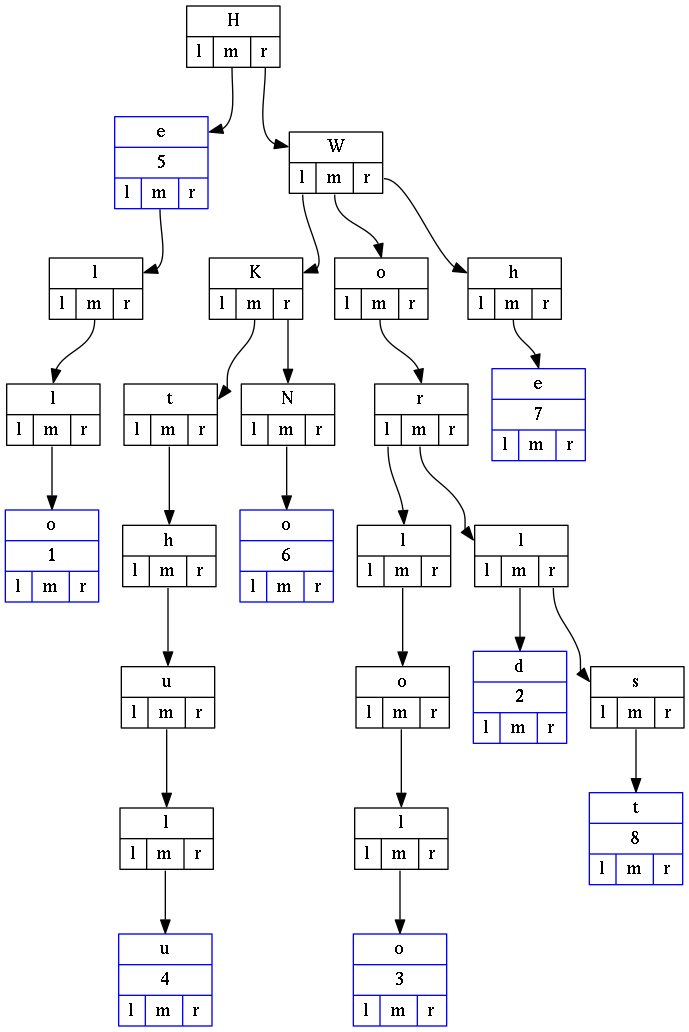
\includegraphics[width=0.5\textwidth]{ternary_search_tree}
    \caption{Een ternaire zoekboom voor de volgende woorden: \texttt{Hello, World, Kthulu, Wololo, No, We}. In deze versie hebben de woorden geen afsluitelement.}
    \label{fig:ternary_search_tree}
\end{figure}
\begin{itemize}
    \item Een alternatieve voorstelling van een meerwegstrie.
    \alert De snelste implementatie van een meerwegstrie gebruikt een tabel van $m$ kindwijzers in elke knoop, wat onnodig veel geheugen vereist.
    \item Men gebruikt dan een ternaire zoekboom waarvan elke knoop een \textbf{sleutelelement} bevat.
    \item \textbf{Zoeken} vergelijkt telkens het sleutelelement met het element in de huidige knoop. Er zijn dan drie mogelijkheden:
    \begin{itemize}
        \item Is het zoeksleutelelement kleiner, dan zoeken we verder in de linkse deelboom, met \textbf{hetzelfde zoeksleutelelement}.
        \item Is het zoeksleutelelement groter, dan zoeken we verder in de rechtse deelboom, met \textbf{hetzelfde zoeksleutelelement}.
        \item Is het zoeksleutelelement gelijk, dan zoeken we verder in de middelste deelboom, met het \textbf{volgende zoeksleutelelement}.
    \end{itemize}
    \item Om te voorkomen dat een sleutel geen prefix is van elke andere sleutel, wordt er terug een afsluitkarakter gekozen.
    \item Een zoeksleutel wordt gevonden wanneer we met zijn afsluitelement bij een knoop met datzelfde element uitkomen.
    \item Een ternaire zoekboom behoudt de volgorde van de opgeslagen sleutels.
    \item De \textbf{voordelen} van een ternaire zoekboom:
    \begin{itemize}
        \item Het past zich goed aan bij onregelmatig verdeelde zoeksleutels.
        \begin{itemize}
            \item De Unicode standaard bevat meer dan 1000 karakters, waarvan enkelen heel vaak gebruikt worden. In dit geval zouden meerwegstries ook te veel geheugen nodig hebben voor de tabellen met wijzers.
        \end{itemize}
        \item Zoeken naar afwezige sleutels is efficiënt. Er wordt maar vergelijken met slechts enkele sleutelelementen. Een normale binaire boom vereist $\Omega(\lg n)$ sleutelvergelijkingen.
        \item Complexe zoekoperaties zijn mogelijk zoals sleutels opsporen die in niet meer dan één element verschillen van de zoeksleutel of zoeken naar sleutels waarvan bepaalde elementen niet gespecifieerd zijn.
    \end{itemize}

    \item Mogelijke \textbf{verbeteringen}:
    \begin{itemize}
        \item Het aantal knopen kan beperkt worden door een combinatie te maken van een trie en een patriciatrie: enkel sleutels opslaan in bladeren en knopen met maar één kind samenvoegen. 
        \item De wortel kan vervangen worden door een meerwegstrieknoop, wat resulteert in een tabel van ternaire zoekbomen. 

        Als het aantal mogelijke sleutelelementen $m$ niet te groot is, volstaat een tabel van $m^2$ ternaire zoekbomen, zodat er een zoekboom overeenkomt met elk eerste paar sleutelelementen.
    \end{itemize}
\end{itemize}